\scanpage{90}
% archive foliation: 89
\[
\begin{aligned}
C_{\bar\omega_*}(\underset{\substack{\Vert\\\unsure{\omega_0|\omega_1}}}{\underbrace{\lambda\delta}})
&=\underbrace{\delta\,d\lambda}_{\text{poids }2}+\unsure{\lambda}
\bigl[\underset{\substack{\Vert\\0}}{[\bar\omega_2,\delta]}
+\underset{\substack{\Vert\\+\underbrace{\bar\omega_1\lambda\delta}_{\text{poids }2}}}{[\bar\omega_1,\delta]}
+[\bar\omega_0,\delta]
\end{aligned}
\]
\margin{$\deleted{\unsure{+|-}}\underbrace{2\bar\omega_0\lambda\delta}$}
\[
\begin{aligned}
C_{\bar\omega_*}(\underset{\substack{\Vert\\\lambda\delta}}{\omega_1})
&=\overbrace{\delta\,d\lambda}^{2}
+\overbrace{\underset{\substack{\Vert\\\lambda\delta}}{\omega_1}
(\overbrace{\bar\omega_1}^{2}-2\bar\omega_0)}^{1}\\
C_{\bar\omega_*}(\underset{\substack{\Vert\\\mu.1}}{\omega_0})
&=\overbrace{d\mu}^{1}
+\overbrace{\omega_0(\overbrace{-\bar\omega_2}^{2}+\bar\omega_0)}^{0}\\
C_{\bar\omega_*}(\underset{\substack{\Vert\\\nu\delta^{-1}}}{\omega_{-1}})
&=\overbrace{\delta^{-1}d\nu}^{0}
+\overbrace{\omega_{-1}(\overbrace{2\bar\omega_2}^{1}-\bar\omega_1)}^{0}
\end{aligned}
\]
\margin{\diagram{$\begin{array}{c|ccc}
\mathfrak g:&\Omega&\underset{\substack{\Vert\\O_X}}{\Omega^0}&\Omega^{-1}\\
\mathfrak g\otimes\omega:&\Omega\otimes\uline\omega&\uline\omega&\Omega^{-1}\otimes\uline\omega
\end{array}$}}

On trouve les conditions suivantes (indépendantes du choix du splittage $\ldots$!)
\par \uline{\unsure{tte|toute} connexion $c$ satisfait}
$c(\operatorname{Fil}_i\mathfrak g)\subset\operatorname{Fil}_{i+1}(\mathfrak g\otimes\uline\omega)$
\par par passage au gradué, il induit
\[
c_{i,i+1}:\deleted{\unsure{\operatorname{gr}_i|\operatorname{Fil}_i}}
\operatorname{gr}_i\mathfrak g\longrightarrow
\operatorname{gr}_{i+1}(\mathfrak g\otimes\omega)\simeq\operatorname{gr}_{i+1}(\mathfrak g)\otimes\omega
\]
qui est \uline{linéaire}, de façon précise
\[
\begin{aligned}
c_{1,2}:\operatorname{gr}_1\to\operatorname{gr}_2,&\quad\Omega\longrightarrow\omega
&&\text{i.e. }c_{12}\in\Gamma\Omega^{-1}\otimes\uline\omega\\
c_{2,3}:\operatorname{gr}_2\to\operatorname{gr}_3,&\quad O_X\longrightarrow\Omega^{-1}\otimes\omega
&&\text{i.e. }c_{23}\in\Gamma\Omega^{-1}\otimes\uline\omega.
\end{aligned}
\]
on a $[c_{12}=-2\bar\omega_0,\ c_{2,3}=\bar\omega_0,\ \text{donc}]$
\[
\boxed{c_{1,2}=-2c_{2,3}}
\]
\figure{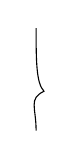
\begin{tikzpicture}\draw (0,0) .. controls (0,-.4) and (0,-.7) .. (.1,-.8)
.. controls (-.1,-.9) and (0,-1) .. (0,-1.3);\end{tikzpicture}}

\uline{NB} On trouve que la connexion respecte la filtration ssi
$\uline{c_{2,3}}=0$ (d'où $c_{1,2}=0$)
[ceci signifie: $\bar\omega_0=0$] ---
\deleted{\unsure{celles qui les}}
\inserted{ce sont aussi}
celles qui respectent le Borel $\mathcal L\subset\mathfrak g$,
i.e. encore celles qui respectent la section $\sigma$ de $P$, i.e. pour lesquelles
$\sigma$ est horizontale. Elles sont \unsure{différentiées|définies par}
une section de $\mathcal L\otimes\omega$.
\par \deleted{\unsure{Or $C$ est bien déterminé!, par des|Or $C$ est bien déterminé!, des}}

\margin{Re \uline{NB} On pourrait considérer
\diagram{\begin{tikzcd}
c^\Omega:\underset{\substack{\simeq\\\mathcal L^\vee\simeq\mathcal L\otimes\Omega^{-1}}}{\mathfrak g/\Omega}
\arrow[r]&\Omega^{-1}\otimes\uline\omega
\end{tikzcd}}
induit par $c$, \unsure{induisant $i$ (linéaire)|et devant être linéaire})
sur $\Omega^0\simeq O_X\subset\mathcal L\otimes\Omega^{-1}$.
Sa connaissance est \uline{équivalente} à celle de $C_\Omega$ si $2$ inv.,
et dans le cas général (p.e. en Car. $2$?) c'est \unsure{peut-être|encore} plus précis $\ldots$}
\figure{\begin{tikzpicture}[x=1cm,y=1cm]
\draw (0,2.3) .. controls (-.2,1.8) and (-.1,.4) .. (0,0)
.. controls (2,-.1) and (4,-.1) .. (6,-.3);
\draw[->] (-2,1) .. controls (-1.4,1.4) and (-.8,1.8) .. (-.5,2);
\end{tikzpicture}}

\uline{NB} Les connexions sur $\mathfrak g$ compatibles avec
crochet \deleted{\unsure{place|plat}}
(si $2$ inv. --- sinon il faut parler des connexions \inserted{\uline{Conn}}
sur $P$, ou $G$ etc) forment un torseur sous $\mathfrak g\otimes\uline\omega$. Or
\diagram{\begin{tikzcd}
{}\arrow[r,Rightarrow]&\mathfrak g\otimes\uline\omega\arrow[r]&\Omega^{-1}\otimes\uline\omega
\end{tikzcd}}
d'où un torseur sous $\Omega^{-1}\otimes\uline\omega$.
\uline{Ce dernier} est splitté canoniquement, i.e. on a
\diagram{\begin{tikzcd}
\uline{\mathrm{Conn}}\arrow[r,"\bar\omega_0"]&\Omega^{-1}\otimes\omega
\end{tikzcd}}
compatible avec $\unsure{\alpha|a}$, et si $c$ section de \uline{Conn},
$\bar\omega_0(c)$ détermine les hom
$\operatorname{gr}_i\mathfrak g\to\operatorname{gr}_{i+1}(\mathfrak g\otimes\uline\omega)$
\diagram{\begin{tikzcd}
\Omega=\operatorname{gr}_1(\mathfrak g)\arrow[r,"-2\bar\omega_0"']&
\omega\simeq\operatorname{gr}_2(\mathfrak g\otimes\unsure{\Omega|\omega})\\
\Omega^0\simeq O_X=\operatorname{gr}_2(\mathfrak g)\arrow[r,"\bar\omega_0"']&
\Omega^{-1}\otimes\uline\omega=\operatorname{gr}_3(\mathfrak g\otimes\uline\omega)
\end{tikzcd}}

Si on considère les $c$ pour lesquels
$\bar\omega_0(c)\in\underset{\substack{\Vert\\\operatorname{Hom}(\Omega,\uline\omega)}}{\Gamma\Omega^{-1}\otimes\uline\omega}$
est donné \inserted{$i$}, on donne une restriction
du Gr. struct. de \uline{Conn} à $\mathcal L\otimes\uline\omega$,
d'où torseur $\mathrm{Conn}_i$ sous $\mathcal L\otimes\uline\omega$. Or on a
\diagram{\begin{tikzcd}\mathcal L\otimes\uline\omega\arrow[r]&\uline\omega\end{tikzcd}}
d'où un torseur associé sous $\uline\omega$: les conn.
sur $\mathfrak g$ compatibles avec $i$, \uline{modulo} \inserted{\unsure{q.d.|i.e.}}
ajouter une section de $\Omega\otimes\uline\omega\subset\mathcal L\otimes\uline\omega\subset\mathfrak g\otimes\uline\omega$.
C'est aussi (\deleted{évidemment}) le torseur des restrictions
à $\Omega$ des conn. compatibles avec $i$, ou encore
des hom. additifs op. diff. d'ordre $1$ (rel. $S$
\diagram{\begin{tikzcd}\Omega\arrow[r,"C_\Omega"]&\mathcal L\otimes\omega\end{tikzcd}}
\unsure{telles|tels} que la composée
\diagram{\begin{tikzcd}
\deleted{\unsure{\mathcal L|\Omega}}\Omega\arrow[r,"C_\Omega"]&
\mathcal L\otimes\omega\arrow[r]&\omega
\end{tikzcd}}
soit linéaire (et égale à $-2i$), et que l'on ait
\[
C_\Omega(f\omega)-fC_\Omega(\omega)\simeq\omega\otimes df.
\qquad\begin{array}{l}\omega\in\Gamma\Omega\\f\in\Gamma O_X\end{array}
\]
\figure{\begin{tikzpicture}[x=1cm,y=1cm]
\draw (0,0)--(.05,.7)--(3.1,.7)--(3.3,0);
\draw (4,6)--(4.1,1);
\end{tikzpicture}}
\margin{verso}
\figure{\begin{tikzpicture}[x=1cm,y=1cm]
\draw (0,0)--(0,-.8);\draw (.07,.06)--(.07,-.7);
\draw (5,0)--(5,-.8);\draw (5.07,.06)--(5.07,-.7);
\end{tikzpicture}}

